\clearpage
\section{Spatial Decomposition via Equivalent Network Approximation (ENApp)}

\subsection{Introduction and Motivation}

Optimal power flow (OPF) methods are employed to optimally coordinate grid's controllable resources for different system-level objectives, such as economic operations, reliability, and resilience. The significance of OPF studies is growing in relevance at the distribution system level, driven by the increasing adoption of distributed energy resources (DERs), particularly photovoltaic systems (PVs) and battery energy storage systems (BESS). Furthermore, the adoption of BESS is gaining significance for managing the variability of DERs through controlled charging and discharging, thereby ensuring supply-demand balance \cite{tgangwar}. Incorporating BESS into OPF problems substantially raises the complexity of network optimization problems, transitioning from a single-period, time-decoupled OPF to a multi-period, time-coupled OPF.

Traditionally, centralized OPF (COPF) methods have been widely used, where a central controller processes aggregated grid-edge data, executes the OPF algorithm, and sends control signals to manage resources \cite{spaul}. The COPF algorithms for DER management are generally developed as a mixed integer non-convex programming (MINCP) problem and then simplified either as a convex problem by adopting second-order cone programming (SOCP) relaxations \cite{Wei} \cite{Chowdhury}, or as a linear problem by adopting Taylor series expansion \cite{spaul}, polyhedral approximations \cite{Guo} or linear power flow models \cite{Yuan}. Unfortunately, COPF methods pose scalability challenges for larger networks and for difficult classes of OPF problems such multi-period time-coupled formulations required to optimally manage BESS. 

To address scalability challenges, distributed OPF (DOPF) algorithms have been introduced. These algorithms decompose the COPF problem into smaller sub-problems that are solved concurrently, leveraging communication among neighboring areas. In this context, the Auxiliary Problem Principle (APP) and the Alternating Direction Method of Multipliers (ADMM) are widely adopted algorithms for solving various OPF problems, including non-convex formulations \cite{Fazio}, convex-relaxed versions \cite{Zheng, Wang, Biswas}, and linear approximations \cite{Paul2}. Similarly, in a prior study \cite{Sadnan}, the authors' research group introduced a DOPF framework utilizing the Equivalent Network Approximation method (ENApp). This approach was shown to require fewer macro iterations compared to traditional ADMM or APP algorithms for solving DOPF problems.

The above references \cite{Wei}-\cite{Paul2} mainly focused on solving single time-period OPF problems and did not include the coordination of grid-edge devices that introduce time-coupled constraints, such as BESS. The inclusion of BESS models results in a multi-period OPF (MPOPF) problem with time-coupled constraints. Reference \cite{Gabash} proposed a nonlinear multi-period centralized OPF (MPCOPF) approach to optimally coordinate active-reactive power dispatch from batteries and DERs in distribution systems. Alizadeh and Capitanescu \cite{Alizadeh} proposed a stochastic security-constrained MPCOPF, which sequentially solves a specific number of linear approximations of the original problem. Usman and Capitanescu \cite{Usman} developed three different MPCOPF frameworks. All three approaches begin by solving a linear program to optimize the binary variables first, followed by either a linear or non-linear program to optimize the continuous variables. Optimal battery schedules are determined in \cite{Aghdam} considering uncertain renewable power generation by solving an MPCOPF. A bi-level robust MPCOPF is suggested in \cite{Zhang1} for determining active and reactive power dispatches from the grid edge devices. Wu et al. \cite{Wu} framed a Benders Decomposition (BD) based multi-period distributed OPF (MPDOPF) after decomposing the original centralized multi-parametric quadratic problem into one master and multiple sub-problems. 

Over recent years, numerous research efforts have focused on developing MPOPF methodologies. However, the following research gaps persist:
\begin{enumerate}
    \item The MPOPF models are mainly solved centrally \cite{Gabash}-\cite{Zhang1}. The centralized methods suffer from scalability and computational challenges, requiring significantly long solution times, rendering them unsuitable for operational decision-making.
    \item Reference \cite{Wu} proposed a MPDOPF framework using Benders Decomposition. However, this approach suffers from slow convergence and needs a central controller to solve the master problem. 
\end{enumerate}

This work aims to address the above research gaps by developing a spatially distributed MPOPF (MPDOPF) framework. The distribution system is divided into multiple connected areas, each solving its own local MPOPF problem and periodically communicating the values of boundary variables with neighboring areas. The interaction between the areas is modeled by following the principles of the ENApp DOPF algorithm. ENApp outperforms the other DOPF algorithms in terms of convergence speed and requires fewer macro iterations \cite{Sadnan}. The specific contributions of this work are listed below:
\begin{enumerate}
    \item A MPOPF framework is proposed for distribution systems consisting of DERs and batteries. The integer variables related to battery charging/discharging are avoided by adding a ``Battery Loss'' cost term in the objective function. The loss term will ensure the non-occurrence of simultaneous charging/discharging operations.
    \item The original MPOPF framework is solved in a distributed manner by following the principles of the ENApp-based distributed OPF. This provides faster convergence and requires less solution time compared to the traditional MPCOPF.
    \item Detailed comparative analyses between traditional MPCOPF and the proposed MPDOPF are done using the IEEE 123 bus test system and the benefits of the proposed approach are demonstrated. ACOPF feasibility validation is also performed by implementing the derived controls into an OpenDSS model of the test system.
\end{enumerate}

\subsection{Problem Formulation}

\subsubsection{Notations}
In this study, the distribution system is modeled as a tree (connected graph) with $N$ number of buses (indexed with \(i\), \(j\), and \(k\)); the study is conducted for $T$ time steps (indexed by $t$), each of interval length $\Delta t$. The sets of buses with DERs and batteries are $D$ and $B$ respectively, such that $D, B \subseteq N$.
A directed edge from bus $i$ to $j$ in the tree is represented by $ij$ and the set for edges is given by $\mathcal{L}$. Line resistance and reactance are \(r_{ij}\) and \(x_{ij}\), respectively. Magnitude of the current flowing through the line at time \(t\) is denoted by \(I_{ij}^t\) and  $l_{ij}^t=\left(I_{ij}^t\right)^2$. The voltage magnitude of bus \(j\) at time \(t\) is given by \(V_j^t\) and  $v_j^t=\left(V_j^t\right)^2$. Apparent power demand at a node \(j\) at time \(t\) is \(s^t_{L_j}\) (\(=p^t_{L_j}+\textit{j}q^t_{L_j}\)). The active power generation from the DER present at bus \(j\) at time \(t\) is denoted by \(p^t_{D_j}\) and controlled reactive power dispatch from the DER inverter is \(q^t_{D_j}\). DER inverter capacity is $S_{D_{R_j}}$.
The apparent power flow through line {\(ij\)} at time \(t\) is \(S_{ij}^t\) (\(=P_{ij}^t+\textit{j}Q_{ij}^t\)). The real power flowing from the substation into the network is denoted by $P^t_{Subs}$ and the associated cost involved per kWh is $C^t$. The battery energy level is \(B_j^t\). Charging and discharging active power from battery inverter (of apparent power capacity $S_{B_{R_j}}$) are denoted by \(P_{c_j}^t\) and \(P_{d_j}^t\), respectively and their associated efficiencies are $\eta_c$ and $\eta_d$, respectively. The energy capacity of the batteries is denoted by $B_{R_j}$, and the rated battery power is $P_{B_{R_j}}$. $soc_{min}$ and $soc_{max}$ are fractional values for denoting safe soc limits of a battery about its rated state-of-charge (soc) capacity. The reactive power support of the battery inverter is indicated by \(q_{B_j}^t\). 

\subsubsection{MPCOPF with Batteries}
The OPF problem aims to minimize two objectives as shown in \cref{eq:genCost_withSCD_enapp}. The first term in \cref{eq:genCost_withSCD_enapp} aims to minimize the total energy cost for the entire horizon. Including the `Battery Loss' cost as the second term ($\alpha > 0$) helps eliminate the need for binary (integer) variables typically used to prevent simultaneous charging and discharging. The resulting OPF problem is a non-convex optimization problem \cite{Nazir2021Sep}.

\begin{equation}
    \begin{split}
        \min \sum_{t = 1}^{T} \left[ C^t P^t_{Subs} \Delta t+ \alpha \sum_{j \in \mathcal{B}} \left\{ (1-\eta_C)P^t_{C_j} \right. \right. \\
        \left. \left. + \left( \frac{1}{\eta_D} - 1 \right) P^t_{D_j} \right\} \right]
    \end{split}
    \label{eq:genCost_withSCD_enapp}
\end{equation}


Subject to the constraints \crefrange{eq:RealPowerBalanceNodej_enapp}{eq:modelEndsHere-and-lim_Bj_enapp} as given below:

\begin{align}
    {\sum_{(j, k) \in \mathcal{L}} \left\{P_{jk}^t\right\} 
    - \left(P_{ij}^t - r_{ij}l_{ij}^t\right)} &= {\left(P_{d_j}^t - P_{c_j}^t\right)} \nonumber \\[-0.8em]
    {} & {\qquad  + p^t_{D_j} - p^t_{L_j}}
    \label{eq:RealPowerBalanceNodej_enapp} &&
\end{align}

\vspace{-2.0em}

\begin{align}
    {\sum_{(j, k) \in \mathcal{L}} \left\{Q_{jk}^t\right\}  
    - \left(Q_{ij}^t - x_{ij}l_{ij}^t\right)} &= {q_{D_j}^t + q_{B_j}^t - q^t_{L_j}}
    \label{eq:ReactivePowerBalanceNodej_enapp}
\end{align}

\vspace{-1.5em}

\begin{align}
    {v_j^t} &= {v_{i}^t - 2(r_{ij}P_{ij}^t + x_{ij}Q_{ij}^t) + \left\{r_{ij}^2 + x_{ij}^2\right\}l_{ij}^t}  
    \label{eq:KVL-branch-ij_enapp} &&
\end{align}

\vspace{-1.5em}

\begin{align}
    {(P_{ij}^{t})^2 + (Q_{ij}^{t})^2} &= {l_{ij}^t v_i^t} 
    \label{eq:ApparentPowerEquationBFM_enapp} &&
\end{align}

\vspace{-2.0em}

\begin{align}
    {P^t_{Subs}} &\geq {0} \label{eq:substationRealPowerLimits_enapp} &&
\end{align}

\vspace{-2.0em}

\begin{align}
    { v^{t}_{j} } &\in { \left[ V^{2}_{min}, V^{2}_{max} \right]} \label{eq:lim_vj_enapp} &&
\end{align}

\vspace{-1.5em}

\begin{align}
    { q^{t}_{D_{j}} } 
    &\in
    { \left[-\sqrt{ {S_{D_{R, j}}}^2 - {p^{t}_{D_{j}}}^2}, \sqrt{ {S_{D_{R, j}}}^2 - {p^{t}_{D_{j}}}^2}\right] } \label{eq:qDj_enapp} &&
\end{align}

\vspace{-1.5em}

\begin{align}
    {B_{j}^{t}} &= {B_{j}^{t-1} + \Delta t  \eta_c P_{c_j}^t - \Delta t\frac{1}{\eta_d} P_{d_j}^t } \label{eq:SOC-j_enapp} &&
\end{align}

\vspace{-1.5em}

\begin{align}
    { P^{t}_{c_{j}}, P^{t}_{d_{j}} }
    &\in
    { \left[ 0, P_{B_{R_{j}}} \right]}, \quad B_{j}^{0}=B_{j}^{T} \label{eq:lim_PcPdj_enapp} &&
\end{align}

\vspace{-1.5em}

\begin{align}
    { q^{t}_{B_{j}} } 
    &\in 
    { \left[-\sqrt{0.44}P_{B_{R, j}}, \sqrt{0.44}P_{B_{R, j}}\right] } \label{eq:qBj_enapp} &&
\end{align}

\vspace{-1.5em}

\begin{align}
    { B^{t}_{j} } &\in { \left[ soc_{min}B_{R, j}, soc_{max}B_{R, j} \right] } \label{eq:modelEndsHere-and-lim_Bj_enapp} &&
\end{align}

A branch power flow model, given by \crefrange{eq:RealPowerBalanceNodej_enapp}{eq:ApparentPowerEquationBFM_enapp}, is used to represent power flow in distribution system. Constraints \cref{eq:RealPowerBalanceNodej_enapp,eq:ReactivePowerBalanceNodej_enapp} model the active and reactive power balance at node $j$, respectively.
The KVL equation for branch $(ij)$ is represented by \cref{eq:KVL-branch-ij_enapp}, while the equation describing the relationship between current magnitude, voltage magnitude and apparent power magnitude for branch $(ij)$ is given by \cref{eq:ApparentPowerEquationBFM_enapp}. Backflow of real power into the substation from the distribution system is avoided using the constraint \cref{eq:substationRealPowerLimits_enapp}. The allowable limits for bus voltages are modeled via \cref{eq:lim_vj_enapp}. \cref{eq:qDj_enapp} describes the reactive power limits of DER inverters. The trajectory of the battery energy versus time is given by \cref{eq:SOC-j_enapp} (this is a time-coupled constraint). Battery charging and discharging powers are limited by the battery's rated power capacity, as given by \cref{eq:lim_PcPdj_enapp}. \cref{eq:lim_PcPdj_enapp} also says that the initial and final energy levels for battery must be the same at the end of the optimization time horizon. Every battery's reactive power is also constrained by the corresponding inverter's rated capacity, modeled in \cref{eq:qBj_enapp}. For the safe and sustainable operation of the batteries, the energy $B^{t}_{j}$ is constrained to be within some percentage limits of the rated battery SOC capacity, modeled using \cref{eq:modelEndsHere-and-lim_Bj_enapp}.

\subsubsection{ENApp-based MPDOPF with Batteries} \label{subsec:ENApp}
Assuming the presence of a feasible solution for the MPCOPF problem, the MPDOPF is formulated by decomposing the distribution system into multiple small areas. In this paper, the interaction between the two areas will follow the principle of ENApp algorithm. The ENApp algorithm leverages the radial topology of the distribution network to solve the network-level optimization problem in a distributed manner. Each area has a local controller (LC) that solves its specific local optimization problem. The local optimization problem will be the same MPOPF as described in Section II-B but defined using only the variables and parameters specific for the corresponding area. The boundary buses between two areas are accounted as voltage sources for downstream areas and load buses for upstream areas. By knowing the upstream voltage and downstream load data, the LCs will solve their area-specific MPOPF in parallel. Once LC problem converges, the downstream and upstream LCs inform power flows and voltage data to their respective upstream and downstream areas. The LCs will again solve their local MPOPF and exchange the updated boundary variables with their neighbors. This iterative process terminates after a convergence is achieved at all boundary buses. Comprehensive details of the ENApp algorithm are available in \cite{Sadnan}. Note that for the case of multi-period optimization with $T$ time steps, each area exchanges a data vector containing $2T$ boundary variables with its neighboring areas. This includes voltage and power flow data for each of the $T$ time steps. 

\subsection{Case Study Demonstration: IEEE 123 Bus Test System}

\subsubsection{Test System Description}

The case studies are conducted on the balanced three-phase version of the IEEE 123 bus test system, which has $85$ Load Nodes. Additionally, $20 \% \, (17)$ and $30 \% \, (26)$ of these load nodes also contain reactive power controllable PVs and BESS, respectively. Their ratings are as per Table~\ref{table:parameter-values_enapp}. To demonstrate the effectiveness of the proposed algorithm, the test system is divided into four areas as shown in Fig.~\ref{fig:ieee123-four-area-figure}. It is assumed that a horizon-wide forecast for loads $p^t_L$, solar power output $p^t_D$ and cost of substation power  $C^t$ is available to the distribution system operator. Initially, the study is carried out for 5 hours with input data shown in Fig.~\ref{fig:inputCurve-5}. The five-hour workflow is described below. 

\def\ds{\rule{0pt}{1.5ex}}

\begin{table}[t]
    \centering
    \caption{Parameter values}
    \begin{tabular}{|l|c|}
    \hline
    \textbf{Parameter} & \textbf{Value} \\ \hline
    $V_{min}, V_{max}$ & 0.95\, pu, 1.05\, pu \\ \hline
    $p_{\ds D_{R_j}}$ & $0.33 p_{\ds L_{R_j}}$ \\ \hline
    $S_{D_{R_j}}$ & $1.2 p_{\ds D_{R_j}}$ \\ \hline
    $P_{B_{R_j}}$ & $0.33 p_{\ds L_{R_j}}$ \\ \hline
    $S_{B_{R_j}}$ & $1.2 P_{\ds B_{R_j}}$ \\ \hline
    $B_{R_j}$ & $T_{fullCharge} \times P_{B_{R_j}}$ \\ \hline
    $T_{fullCharge}$ & 4 h \\ \hline
    $\Delta t$ & 1 h \\ \hline
    $\eta_c, \eta_d$ & 0.95, 0.95 \\ \hline
    $soc_{min}, soc_{max}$ & 0.30, 0.95 \\ \hline
    $\alpha$ & 0.001 \\ \hline
    \end{tabular}
    \label{table:parameter-values_enapp}
\end{table}

\begin{figure}[t]
    \centering
    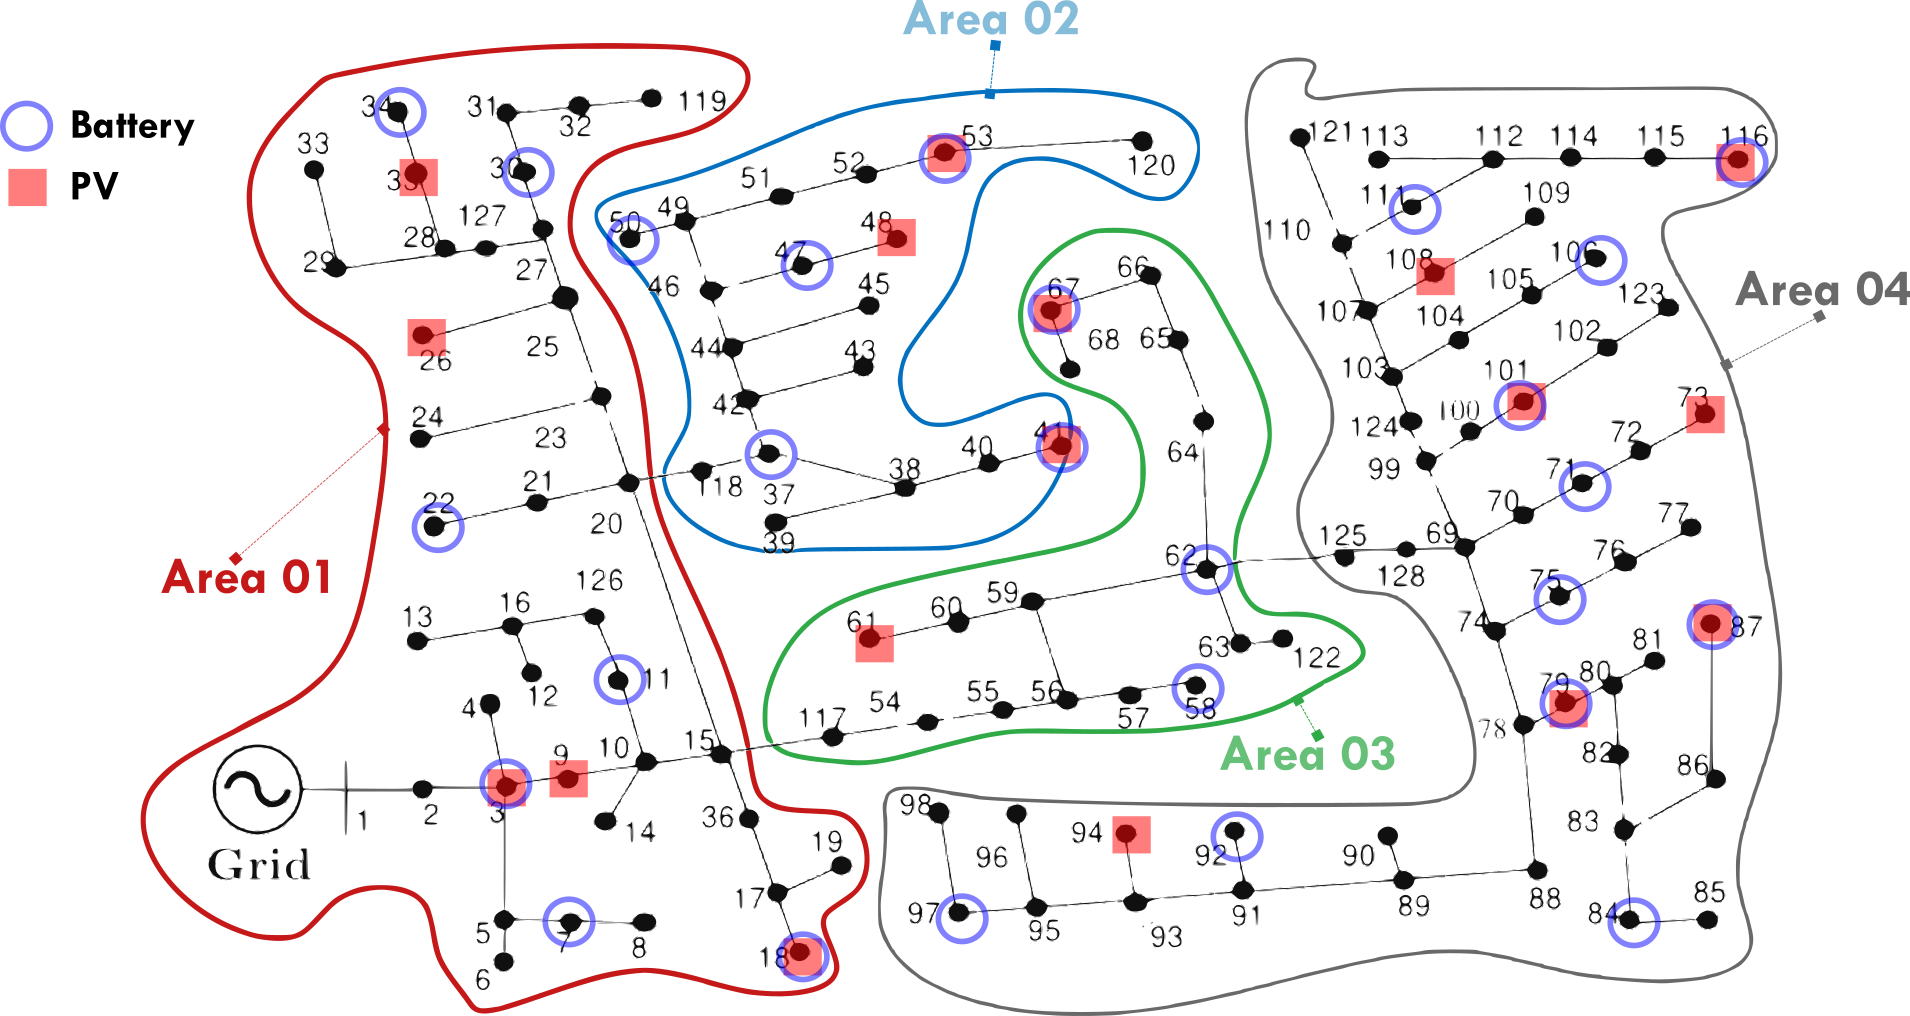
\includegraphics[width=\linewidth]{figures/ieee123-FourAreas-pv20-batt30.png}
    \caption{IEEE 123 node system divided into four areas}
    \label{fig:ieee123-four-area-figure}
    \vspace{-4mm}
\end{figure}

\begin{figure}[t]
    \centering
    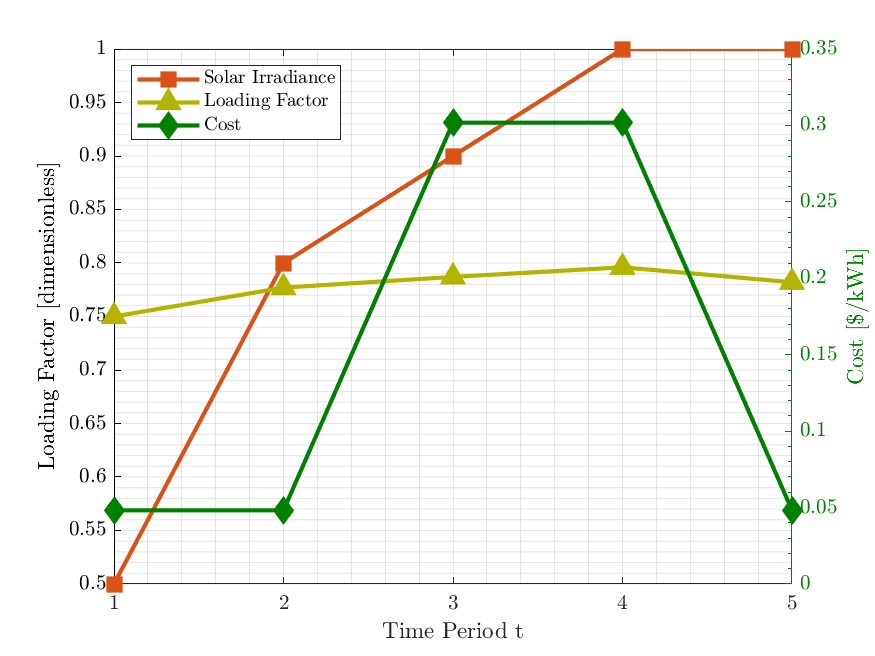
\includegraphics[height=0.25\textheight]{figures/T5-inputCurves/InputCurves_Horizon_5.png}
    \caption{Forecasts for demand power, irradiance and cost of substation power over a 5 hour horizon}
    \label{fig:inputCurve-5}
    \vspace{-4mm}
\end{figure}

\subsubsection{Simulation Workflow}

All simulations were set up in MATLAB 2023a including both the high level algorithms as well as calls to the optimization solver. MATLAB's \texttt{fmincon} function was used to parse the nonlinear nonconvex optimization problem described by \crefrange{eq:genCost_withSCD_enapp}{eq:modelEndsHere-and-lim_Bj_enapp} in tandem with the SQP optimization algorithm to solve it. From the completed simulations, the resultant optimal control variables were obtained, and were passed through an OpenDSS engine (already configured with system data and forecast values) in order to check for the ACOPF feasibility of the results. 
The associated code may be found in \cite{MPOPFRepo}. 
As the IEEE 123 bus system is decomposed into 4 areas, so the total number of variables exchanged at each iteration for the 5-hour simulation of the MPDOPF is \(2*3*5=30\).

\subsection{Simulation Results and Performance Analysis}

In the following subsections, the proposed MPDOPF algorithm is compared against the MPCOPF algorithm in terms of resultant optimal control variables, optimality gap in the objective function, and computational performance. Secondly, the resultant control variables are tested for ACOPF feasibility against OpenDSS. Section~\ref{subsec:simulationResults_enapp} describes the comparison over a $5$ hour horizon with an additional focus on describing the workflow of the MPDOPF algorithm. Section~\ref{subsec:scalabilityAnalysis_enapp} describes the comparison over a $10$ hour horizon to test for the scalability of the MPDOPF algorithm.

\subsubsection{5-Hour Horizon Results} \label{subsec:simulationResults_enapp}

Table~\ref{table:opt-5-20-30_enapp} depicts a comparison between MPCOPF and MPDOPF in their problem scope, results and computational performance.

\paragraph{Largest Subproblem vs. Computational Performance}
This first section of the Table~\ref{table:opt-5-20-30_enapp}, `largest subproblem' provides specifics of the `computational bottleneck' encountered by either algorithm during its course. As described in Section~\ref{subsec:ENApp}, the bottleneck represents the OPF subproblem which is computationally the most intensive and thus is a key indicator of the expected time the algorithm will take to complete. As can be seen in the third section `Computation', there is more than a $10$x speedup in computation time with MPDOPF, even though $5$ such iterations were performed, totalling to $20$ OPF calls over the $4$ areas of the test system.      

\paragraph{Optimality of Objective Function and Control Variables}
The second section of the Table~\ref{table:opt-5-20-30_enapp} i.e. `Simulation results' showcases that MPDOPF provides almost zero optimality gap (same values for Substation Power Cost, the objective function). Interestingly, there is a significant difference in the suggested optimal reactive power control values for inverters associated with DERs and batteries (results aggregated over all components over the horizon for conciseness). This highlights the fact that a nonconvex nonlinear optimization problem may not necessarily have a unique global optimal point. There is a possibility of having multiple feasible solutions with the same objective function value. 

\begin{table}[t]
    \centering
    \caption{Comparative analyses between MPCOPF and MPDOPF - $5$ time-period horizon}
    \begin{tabular}{|l|c|c|}
    \hline
    \textbf{Metric} & \textbf{MPCOPF} & \textbf{MPDOPF} \\ \hline
    Largest subproblem & \multicolumn{2}{c|}{} \\ \hline
    \quad Decision variables & {3150} & {1320} \\ \hline
    \quad Linear constraints & {5831} & {2451} \\ \hline
    \quad Nonlinear constraints & {635} & {265} \\ \hline
    Simulation results  & \multicolumn{2}{c|}{} \\ \hline
    \quad Substation power cost (\$) & 576.31 & 576.30 \\ \hline
    \quad Substation real power (kW) & 4308.28 & 4308.14 \\ \hline
    \quad Line loss (kW) & 75.99 & 76.12 \\ \hline
    \quad Substation reactive power (kVAR) & 574.18 & 656.24 \\ \hline
    \quad PV reactive power (kVAR) & 116.92 & 160.64 \\ \hline
    \quad Battery reactive power (kVAR) & 202.73 & 76.01 \\ \hline
    Computation  & \multicolumn{2}{c|}{} \\ \hline
    \quad Number of Iterations & - & 5 \\ \hline
    \quad Total Simulation Time (s) & 521.25 & 49.87 \\ \hline
    \end{tabular}
    \label{table:opt-5-20-30_enapp}
    \vspace{-3mm}
\end{table}

\paragraph{ACOPF Feasibility Analysis}
Table~\ref{table:feas-5-20-30_enapp} showcases the ACOPF feasibility of the control values suggested by the MPDOPF algorithm. The first section `Full horizon' describes the respective output variables for the entire horizon from MPDOPF and OpenDSS. The second section `Max. all-time discrepancy' stores the highest discrepancy between key state/output variables for all components across any time between MPDOPF and OpenDSS. In both sections, the discrepancies are small enough to warrant the feasibility of the obtained solution. 

\begin{table}[H]
    \centering
    \caption{ACOPF feasibility analyses - $5$ hour}
    \begin{tabular}{|l|c|c|}
    \hline
    \textbf{Metric} & \textbf{MPDOPF} & \textbf{OpenDSS} \\ \hline
    Full horizon  & \multicolumn{2}{c|}{} \\ \hline
    \quad Substation real power (kW) & 4308.14 & 4308.35 \\ \hline
    \quad Line loss (kW) & 76.12 & 76.09 \\ \hline
    \quad Substation reactive power (kVAR) & 656.24 & 652.49 \\ \hline
    Max. all-time discrepancy & \multicolumn{2}{c|}{} \\ \hline
    \quad Voltage (pu) & \multicolumn{2}{c|}{0.0002} \\ \hline
    \quad Line loss (kW) & \multicolumn{2}{c|}{0.0139} \\ \hline
    \quad Substation power (kW) & \multicolumn{2}{c|}{0.3431} \\ \hline
    \end{tabular}
    \label{table:feas-5-20-30_enapp}
    \vspace{-3mm}
\end{table}

To ensure that battery charging and discharging complementarity is respected without relying on integer constraints, the battery charging and discharging profiles were carefully examined. The results confirm this complementarity, as illustrated in Fig.~\ref{fig:batt-plot-dopf-5-20-30-genCost_enapp} as one such example.

\begin{figure}[t]
    \centering
    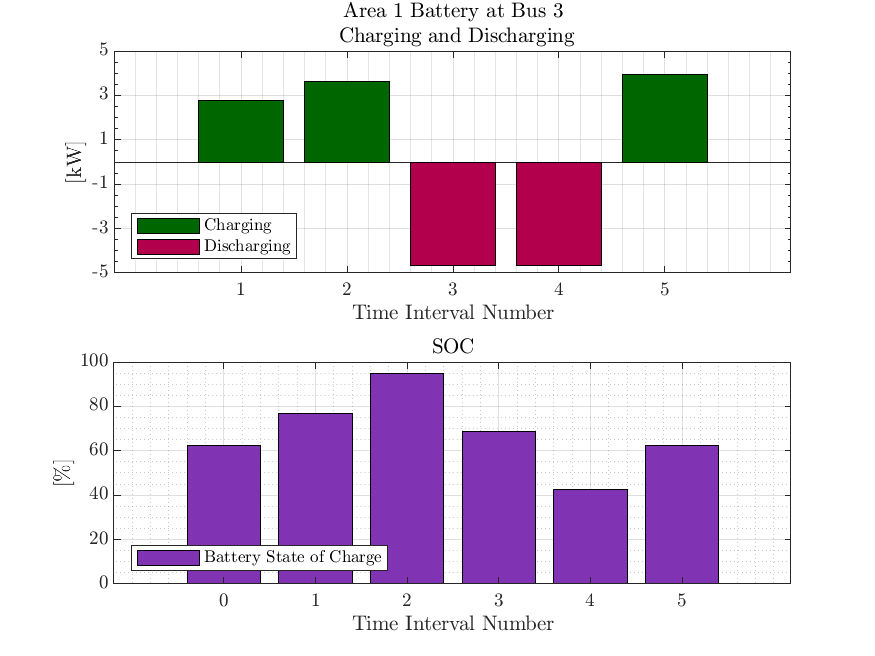
\includegraphics[width=\linewidth]{figures/T5-pv20-batt30-genCost/dopf/BatteryPlots/macroItr_5_genCost_Battery_1_alpha_0.001.png}
    \vspace{-5mm}
    \caption{Charging-discharging and SOC graphs for battery at bus 3 located in Area 1 obtained by MPDOPF}
    \label{fig:batt-plot-dopf-5-20-30-genCost_enapp}
    \vspace{-3mm}
\end{figure}

\paragraph{Workflow Analysis}
The workflow of the MPDOPF algorithm, which involves the exchange of boundary variables between parent-child area pairs, is illustrated in the convergence plots in Figs.~\ref{fig:voltage_1_2_enapp} and \ref{fig:convergenceCurves-5-20-30_enapp}. Each line graph represents a specific time period for both plots. Similarly, Fig.~\ref{fig:outputConvergence-5-pv20-batt30-genCost_enapp} shows the convergence of the objective function towards its optimal value over successive iterations. From these plots, we observe that although the decision variables may initially deviate from their optimal values, they gradually approach optimality with each rolling iteration, converging after 5 macro iterations in this instance.

\begin{figure}[t]
    \centering
    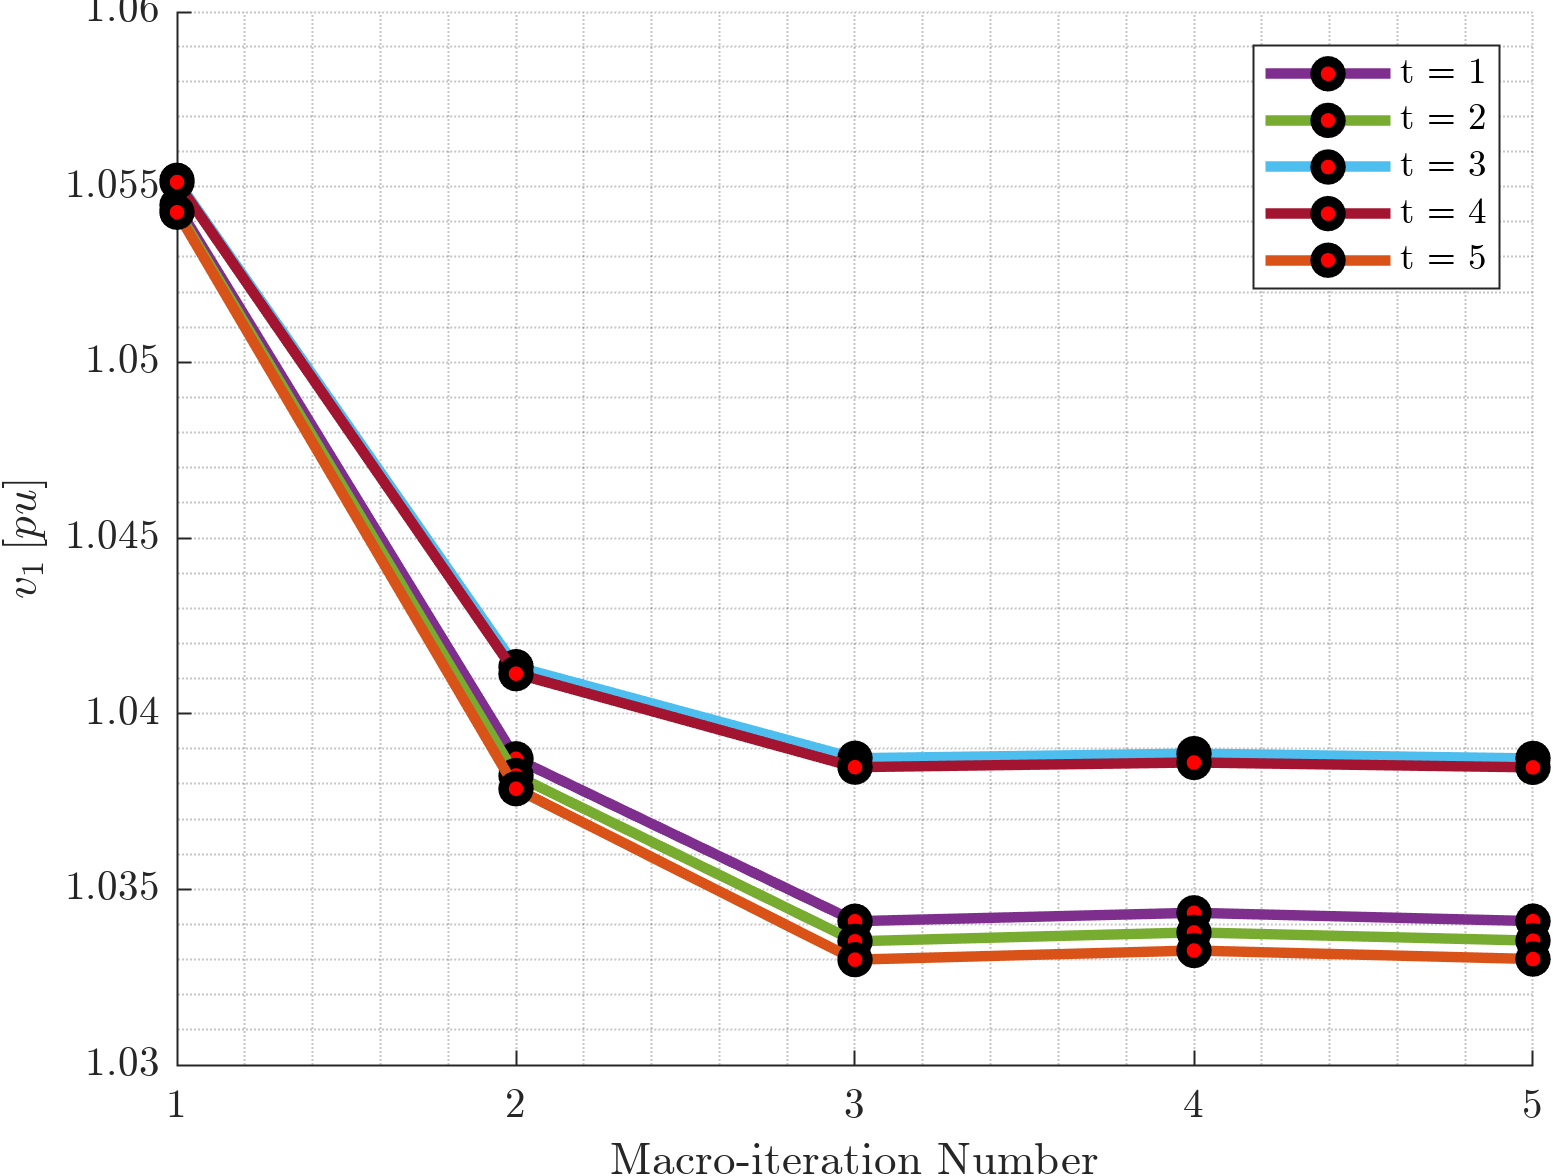
\includegraphics[width=0.8\columnwidth]{figures/T5-pv20-batt30-genCost/dopf/convergenceCurves/BoundaryVoltage_vs_t_vs_macroItr_T_5_Areas_1_2_genCost_pv_20_batt_30_crop.png}
    \caption{Shared voltage data from Area $1$ to Area $2$.}
    \label{fig:voltage_1_2_enapp}
    \vspace{-4mm}
\end{figure}

\begin{figure}[t]
    \centering
    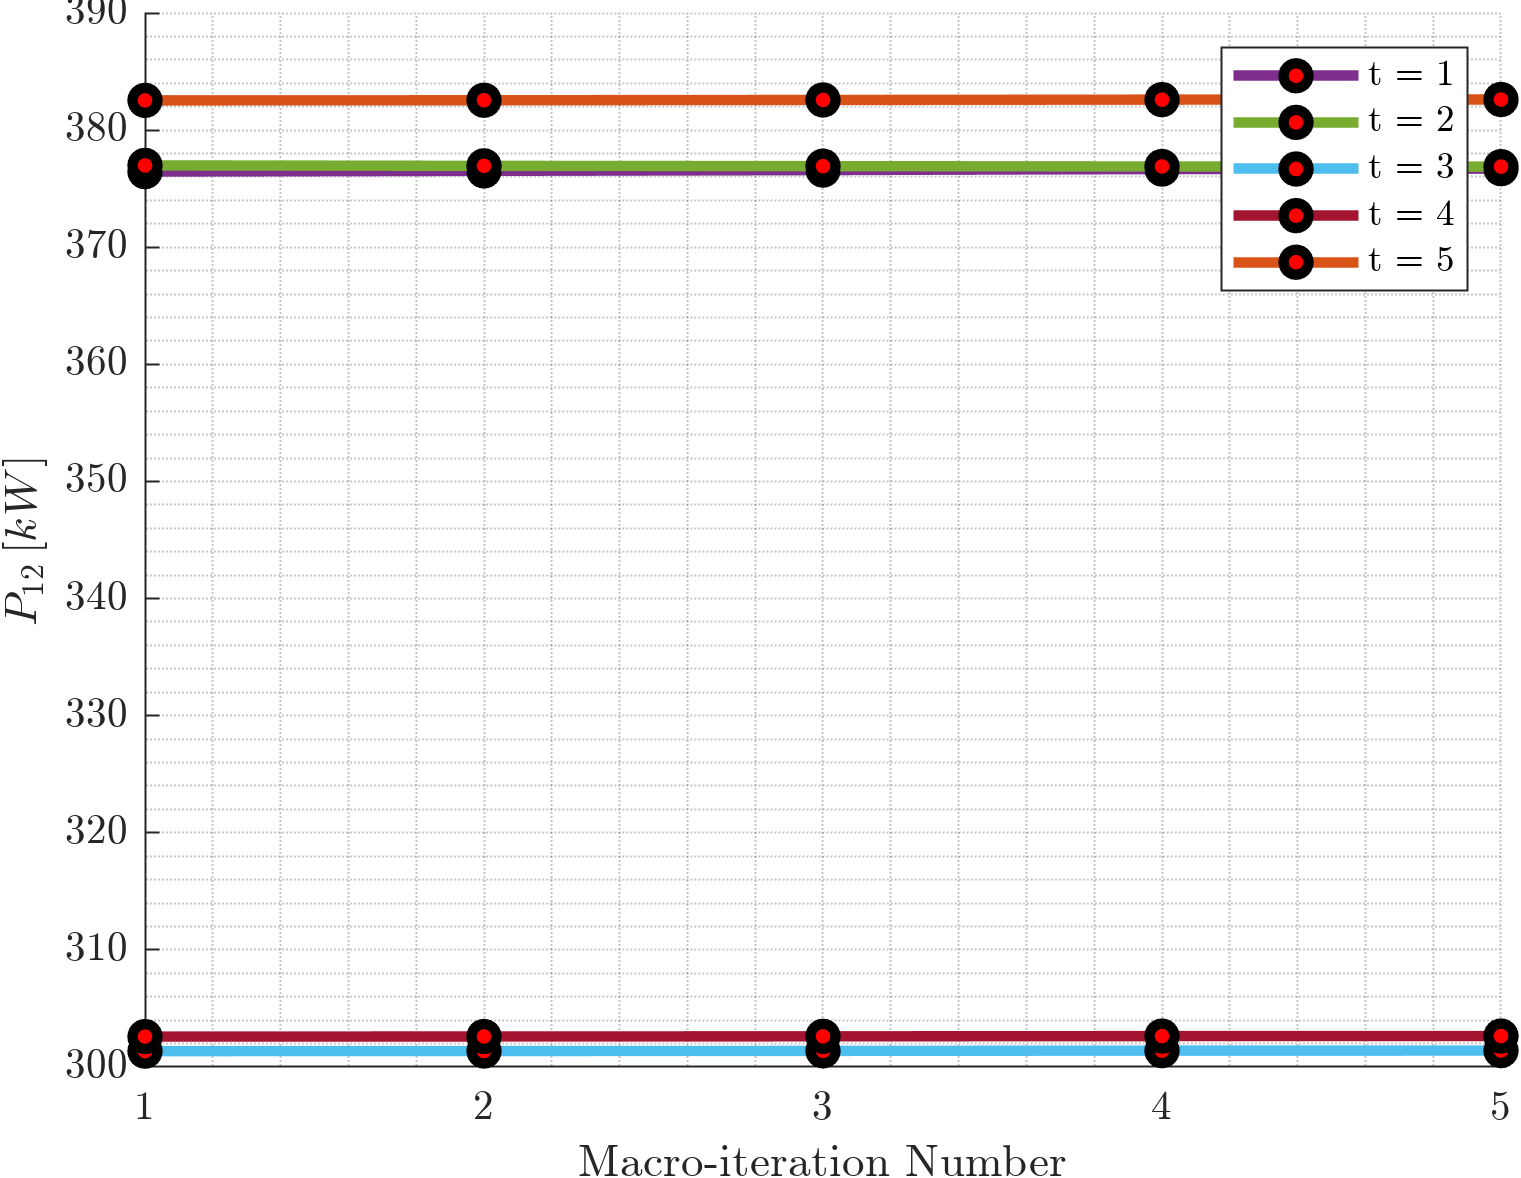
\includegraphics[width=0.8\columnwidth]{figures/T5-pv20-batt30-genCost/dopf/convergenceCurves/BoundaryRealPower_vs_t_vs_macroItr_T_5_Areas_2_4_genCost_pv_20_batt_30_crop.png}
    \caption{Shared real power data from Area $4$ into Area $2$.}
    \label{fig:convergenceCurves-5-20-30_enapp}
    \vspace{-4mm}
\end{figure}

\begin{figure}[t]
    \centering
    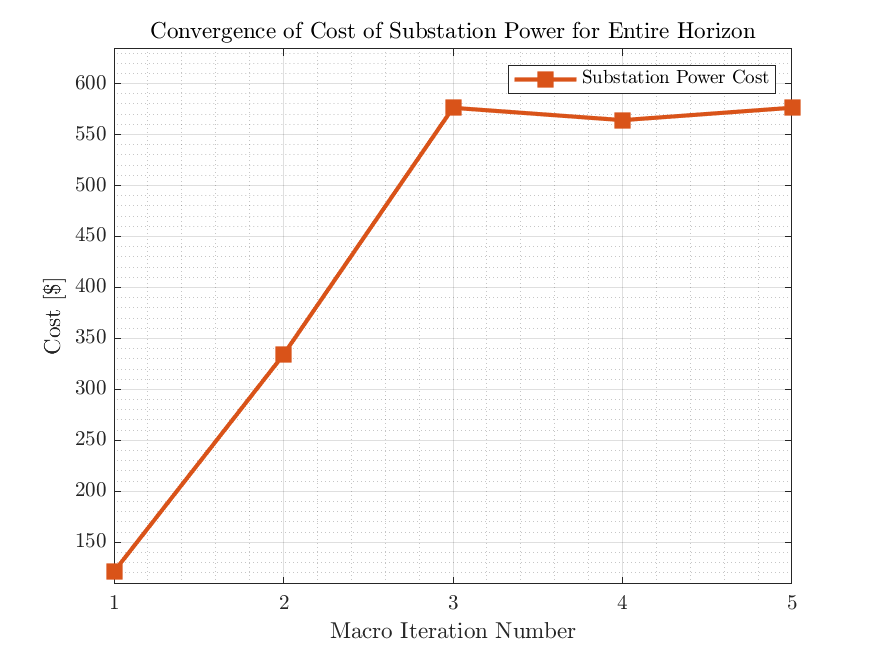
\includegraphics[height=0.25\textheight]{figures/T5-pv20-batt30-genCost/dopf/outputCurves/ObjectiveConvergenceCurves_Horizon_5.png}
    \caption{Convergence of objective function value with each MPDOPF iteration}
    \label{fig:outputConvergence-5-pv20-batt30-genCost_enapp}
    \vspace{-4mm}
\end{figure}

\subsubsection{10-Hour Horizon: Scalability Analysis} \label{subsec:scalabilityAnalysis_enapp}

To demonstrate the scalability of the proposed algorithm, additional simulations were conducted over a 10-hour time horizon. Fig.~\ref{fig:inputCurve-10_enapp} shows the forecasted profiles for load, solar irradiance and cost of substation power over the 10-hour horizon. The simulation results are summarized in Tables~\ref{table:opt-10-20-30_enapp} and \ref{table:feas-copf-10-20-30_enapp}.

From the comparison against MPCOPF in Table~\ref{table:opt-10-20-30_enapp}, it can again be seen that MPDOPF is able to converge to the same optimal solution as MPCOPF. The computational speed up is even more pronounced than for the $5$ time-period simulation. 
It was observed that the solution time for MPCOPF increased significantly with the length of the study horizon, whereas the increase in solution time for MPDOPF was comparatively smaller. This indicates that the proposed spatially distributed MPOPF framework is scalable to a certain extent.

\begin{figure}[t]
    \centering
    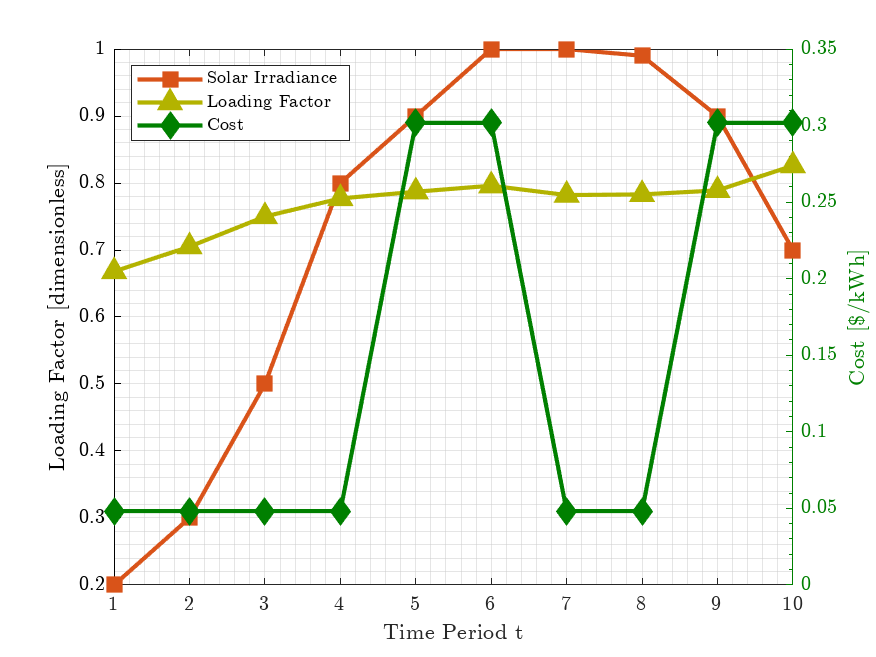
\includegraphics[height=0.25\textheight]{figures/T10-inputCurves/InputCurves_Horizon_10.png}
    \caption{Forecasts for demand power, irradiance and cost of substation power over a 10 hour Horizon}
    \label{fig:inputCurve-10_enapp}
\end{figure}


\begin{table}[H]
    \centering
    \caption{Comparison between MPCOPF and MPDOPF - $10$ hour}
    \begin{tabular}{|l|c|c|}
    \hline
    \textbf{Metric} & \textbf{MPCOPF} & \textbf{MPDOPF} \\ \hline
    Largest subproblem & \multicolumn{2}{c|}{} \\ \hline
    \quad Decision variables & {6300} & {2640} \\ \hline
    \quad Linear constraints & {11636} & {4891} \\ \hline
    \quad Nonlinear constraints & {1270} & {530} \\ \hline
    Simulation results  & \multicolumn{2}{c|}{} \\ \hline
    \quad Substation power cost (\$) & 1197.87 & 1197.87 \\ \hline
    \quad Substation real power (kW) & 8544.28 & 8544.04 \\ \hline
    \quad Line loss (kW) & 148.67 & 148.94 \\ \hline
    \quad Substation reactive power (kVAR) & 1092.39 & 1252.03 \\ \hline
    \quad PV reactive power (kVAR) & 222.59 & 139.81 \\ \hline
    \quad Battery reactive power (kVAR) & 388.52 & 310.94 \\ \hline
    Computation  & \multicolumn{2}{c|}{} \\ \hline
    \quad Number of Iterations & - & 5 \\ \hline
    \quad Total Simulation Time (s) & 4620.73 & 358.69 \\ \hline
    \end{tabular}
    \label{table:opt-10-20-30_enapp}
\end{table}

Again, as can be seen in Table~\ref{table:feas-copf-10-20-30_enapp} comparison against OpenDSS has yielded small discrepancies, attesting to the feasibility of the solution. 

\begin{table}[t]
    \centering
    \caption{ACOPF feasibility analyses - $10$ hour}
    \begin{tabular}{|l|c|c|}
    \hline
    \textbf{Metric} & \textbf{MPDOPF} & \textbf{OpenDSS} \\ \hline
    Full horizon  & \multicolumn{2}{c|}{} \\ \hline
    \quad Substation real power (kW) & 8544.04 & 8544.40 \\ \hline
    \quad Line loss (kW) & 148.94 & 148.87 \\ \hline
    \quad Substation reactive power (kVAR) & 1252.03 & 1243.36 \\ \hline
    Max. all-time discrepancy & \multicolumn{2}{c|}{} \\ \hline
    \quad Voltage (pu) & \multicolumn{2}{c|}{0.0002} \\ \hline
    \quad Line loss (kW) & \multicolumn{2}{c|}{0.0132} \\ \hline
    \quad Substation power (kW) & \multicolumn{2}{c|}{0.4002} \\ \hline
    \end{tabular}
    \label{table:feas-copf-10-20-30_enapp}
    \vspace{-3mm}
\end{table}

\subsection{Summary and Discussion}

The Equivalent Network Approximation (ENApp) approach provides an effective spatial decomposition framework for solving multi-period optimal power flow problems with energy storage in distribution networks. The key advantages of this approach include:

\begin{itemize}
    \item \textbf{Computational Efficiency}: The MPDOPF algorithm achieves more than 10x speedup compared to centralized MPCOPF for medium-sized networks, with the advantage increasing for longer time horizons
    \item \textbf{Scalability}: The computational complexity grows more favorably with network size and time horizon length compared to centralized approaches
    \item \textbf{Distributed Architecture}: Each area solves its local optimization problem independently, enabling parallel computation and reducing the need for centralized data aggregation
    \item \textbf{Solution Quality}: The MPDOPF converges to the same optimal objective value as MPCOPF, with negligible optimality gap
    \item \textbf{ACOPF Feasibility}: The solutions obtained from MPDOPF are validated against OpenDSS, showing excellent agreement with acceptable discrepancies
\end{itemize}

The numerical results on the IEEE 123 bus system demonstrate that ENApp successfully decomposes the spatial network constraints while handling temporal coupling through battery SOC dynamics. The algorithm converges within a few macro iterations (typically 5), and the final solution matches the centralized optimal solution within the specified tolerances. The ACOPF feasibility analysis confirms that the obtained control variables can be implemented in practice with minimal deviation from the desired operating point.

\subsubsection{Key Observations}

Several important observations emerge from the case study results:

\begin{enumerate}
    \item \textbf{Multiple Optimal Solutions}: The nonconvex nature of the MPOPF problem results in multiple feasible solutions with the same objective function value. This is evidenced by the different reactive power dispatch strategies between MPCOPF and MPDOPF, despite achieving the same cost.
    
    \item \textbf{Boundary Variable Convergence}: The convergence plots show smooth and monotonic convergence of boundary variables (voltage and power flow) across area boundaries, indicating stable numerical behavior of the ENApp algorithm.
    
    \item \textbf{Battery Complementarity}: The battery loss cost term successfully prevents simultaneous charging and discharging without requiring integer variables, simplifying the optimization problem while maintaining physical consistency.
    
    \item \textbf{Scalability Advantage}: The computational advantage of MPDOPF becomes more pronounced as the problem size increases (from 5-hour to 10-hour horizon), demonstrating favorable scaling properties.
\end{enumerate}

\subsubsection{Implementation Status and Future Work}

The ENApp-based MPDOPF framework has been successfully implemented and validated on the IEEE 123 bus test system with realistic DER and battery penetrations. The current implementation uses the branch flow model with nonlinear constraints, solved using sequential quadratic programming (SQP) within MATLAB's \texttt{fmincon} solver.

\textbf{Scalability Limitations:} While ENApp achieves 10-13× speedup via spatial decomposition, computational challenges remain for \textit{long time horizons} (e.g., $T > 10$ hours). The coupling across all time periods within each spatial subproblem still requires solving large-scale optimization problems. For planning horizons spanning 24+ hours, spatial decomposition alone proves insufficient. This motivates the need for \textit{temporal decomposition} strategies—the focus of the next chapter—which decompose the time horizon into manageable sub-horizons while maintaining feasibility and near-optimality.

Future extensions of this work will focus on:

\begin{itemize}
    \item \textbf{Larger Networks}: Applying MPDOPF to larger distribution networks (e.g., IEEE 8500 bus system) to further validate scalability
    \item \textbf{Higher DER Penetrations}: Testing the algorithm with increased renewable energy and battery penetrations (e.g., 50\% PV, 50\% BESS)
    \item \textbf{Uncertainty Modeling}: Incorporating stochastic or robust optimization frameworks to handle forecast uncertainties
    \item \textbf{Real-time Applications}: Adapting the algorithm for real-time operational decision-making with rolling horizon optimization
    \item \textbf{Combined Decomposition}: Integrating spatial (ENApp) and temporal (tADMM) decomposition techniques for enhanced scalability in large-scale, long-horizon problems
    \item \textbf{Convergence Acceleration}: Investigating adaptive parameter tuning and warm-start strategies to reduce the number of macro iterations
\end{itemize}

The successful demonstration of ENApp-based MPDOPF on realistic test cases provides a strong foundation for deploying distributed optimization algorithms in operational settings. However, recognizing the complementary need for temporal decomposition leads naturally to the investigation presented in the following chapter.
